\documentclass{article}
\usepackage[margin=2.5cm, top=4cm, headheight=25pt]{geometry}
\usepackage{amsmath, amssymb, enumitem, fancyhdr, graphicx}
\usepackage[indent=20pt]{parskip}
\usepackage[hidelinks]{hyperref}
\usepackage{xcolor}
\usepackage{listings}
\usepackage{subcaption}
\usepackage{url}
\usepackage[most]{tcolorbox}
\usepackage{lastpage}

\tcbuselibrary{listingsutf8} % Support for lstlistings within tcolorbox

\newtcolorbox[auto counter, number within=section]{question}[1][]{%
    colframe=gray!80,                      % Dark gray frame
    colback=gray!5,                       % Light gray background
    coltitle=black,                        % Black title
    title=\textbf{Question~\thetcbcounter}, % Bold title
    fonttitle=\bfseries\large,             % Subtle title font size
    rounded corners,                   % Slightly more rounded corners
    boxrule=0.25mm,                         % Thinner border for a sleek look
    enhanced,                              % Enhanced box features
    attach boxed title to top left={xshift=2mm, yshift=-2mm},
    boxed title style={colframe=gray!80, colback=gray!5, boxrule=0.25mm},
    % Title styling
    #1
}

\bibliographystyle{IEEEtran}
\graphicspath{{./images/}}

% -- Custom Variables --
\def\me{Rajdeep Gill 7934493}
\def\course{ECE 4830}
\def\labsection{B03}
\def\labno{1}
\def\title{Lab 1}

% -- Styling for code snippets --
\lstset{
    basicstyle=\ttfamily\small,           % Basic font style
    keywordstyle=\color{blue},            % Keywords color
    commentstyle=\color{gray},            % Comments color
    stringstyle=\color{teal},             % Strings color
    numbers=left,                         % Line numbers on the left
    numberstyle=\tiny\color{gray},        % Line number style
    stepnumber=1,                         % Line number step
    numbersep=10pt,                       % Space between line numbers and code
    backgroundcolor=\color{lightgray!10}, % Background color
    frame=single,                         % Adds a frame around the code
    breaklines=true,                      % Line breaking for long lines
    captionpos=b,                         % Caption position
    showspaces=false,                     % Don't show spaces
    showstringspaces=false                % Don't show spaces in strings
}
\renewcommand{\lstlistingname}{Code Snippet}

\renewcommand{\arraystretch}{1.2} % For less-ugly tables
\setlength\parindent{0pt}

%----- Samples 
% Questions:
%   \begin{question}[title=Custom Question Title]
%       Question details
%   \end{question}

% Tables:
%   \begin{table}[htbp]
%       \centering
%       \caption{Table Caption}
%       \begin{tabular}{ll}
%           \toprule
%           \textbf{Column 1} & \textbf{Column 2} \\
%           \midrule
%           Row 1 & Row 2 \\
%           Row 3 & Row 4 \\
%           \bottomrule
%       \end{tabular}
%   \end{table} 

% Figures:
%   Single figure:
%       \begin{figure}[htbp]
%           \centering
%           \includegraphics[width=0.5\textwidth]{example-image}
%           \caption{Figure Caption}
%       \end{figure}
%   Multiple figures:
%       \begin{figure}[htbp]
%           \centering
%           \begin{subfigure}[b]{0.5\textwidth}
%               \includegraphics[width=\textwidth]{example-image-a}
%               \caption{First subfigure}
%           \end{subfigure}
%           \begin{subfigure}[b]{0.5\textwidth}
%               \includegraphics[width=\textwidth]{example-image-b}
%               \caption{Second subfigure}
%           \end{subfigure}
%           \caption{Main figure}
%       \end{figure}

\begin{document}

% --------------------------------------------------------------------------------
% TITLE
% --------------------------------------------------------------------------------

\begin{center}
    \huge \title

    \vspace{2mm}
    \hrule

    \vspace{4mm}
    \large \me

    \vspace{2mm}
    \large \course~\labsection

    \vspace{2mm}
    \today
\end{center}

\vspace{4mm}

% --------------------------------------------------------------------------------
% END TITLE
% --------------------------------------------------------------------------------

\newpage

\tableofcontents

\vspace{1cm}
\newpage

\pagestyle{fancy}
\fancyhead[L]{\large Lab \labno}
\fancyhead[R]{\large \me}

\fancyfoot[C]{Page \thepage~of~\pageref{LastPage}}

% --------------------------------------------------------------------------------
% BODY
% --------------------------------------------------------------------------------

\section{Problem 1}
\begin{enumerate}[label=\alph*.]
    \item The provided matlab code generates a signal of 181 samples. The signal consists of a line, unit pulse, sine wave and a random segment. Once the main signal is created, a second signal is created by adding some noise to the main signal. The noise is generated with the \texttt{normrnd} function. The two signals, main and noise, are then plotted on the same graph.

    \item Using ChatGPT to describe the code we get the following response:
    \begin{verbatim}
This MATLAB script generates a synthetic signal composed of linear, constant, 
sinusoidal, and noisy segments to simulate a real-world signal. It introduces 
anomalies, such as spikes and plateaus, and adds Gaussian noise to mimic measurement 
imperfections. The original and noisy signals are plotted side by side, showcasing 
the impact of noise and modifications.
    \end{verbatim}
    This output was the result of the following prompt:
    \begin{verbatim}
        Please describe the provided MATLAB code.
        <<code>>
    \end{verbatim}

    \item Asking an LLM to convert the matlab code to python we get the following response:

    \begin{lstlisting}[language=Python, label={code:p1}, caption={Python code generated by LLM}]
import numpy as np
import matplotlib.pyplot as plt

# Initialize signal
sig = np.zeros(181)

# Signal construction
sig[:51] = np.arange(0, 51)             # Linearly increasing section
sig[51:100] = 50                        # Constant value section
sig[100:125] = 100                      # Higher plateau
sig[125:130] = 0                        # Zero section
sig[130:181] = 50 + 5 * np.random.randn(50)  # Random noisy section

# Append sinusoidal signals
n = np.arange(0, 51)
s1 = 50 + 5 * np.sin(2 * np.pi * 0.1 * n)  # Sine wave 1
s2 = 50 + 5 * np.sin(2 * np.pi * 0.2 * n)  # Sine wave 2
sig = np.concatenate([sig, s1, s2])

# Add baseline offset and anomalies
sig += 50
sig[54:57] = 150  # Spike
sig[58:62] = 125  # Small plateau

# Add noise
xx = np.arange(1, 284)
noisy_sig = sig + np.random.normal(0, 5, size=sig.shape)

# Plot the signals
plt.figure(figsize=(10, 5))
plt.plot(xx, noisy_sig.astype(np.uint8), '--', label='Noisy', linewidth=1.5)
plt.plot(xx, sig.astype(np.uint8), label='Original', linewidth=2)
plt.axis([0, 283, 30, 170])
plt.legend()
plt.xlabel('Index')
plt.ylabel('Signal Value')
plt.title('Original and Noisy Signal')
plt.grid(True)
plt.show()
    \end{lstlisting}
    This output was the result of the following prompt:
    \begin{verbatim}
        Please convert the provided MATLAB code to Python.
        <<code>>
    \end{verbatim}

\item To highlight the transitory parts, we can find the standard deviation of the 30 signals at each sample and plot the results. This will show the parts of the signal that are changing the most.
\end{enumerate}

\section{Problem 2}
\begin{enumerate}[label=\alph*.]
    \item To compute the sampling frequency of the provided signal, we can use the following formula. The signal has 2500 samples, and it is know the signal is 60 Hz, and within the 2500 samples, 6 periods are captured. Therefore, the sampling frequency can be calculated as:
    \begin{align*}
        f_s &= \frac{N}{P} \times f \\
        &= \frac{2500}{6} \times 60 \\
        &= 2500 \times 10 = 25 \text{ kHz}
    \end{align*}
    Labeling the x-axis with the correct time scale instead of the sample number, we get the result shown in \autoref{fig:signal}.
    \begin{figure}[ht!]
        \centering
        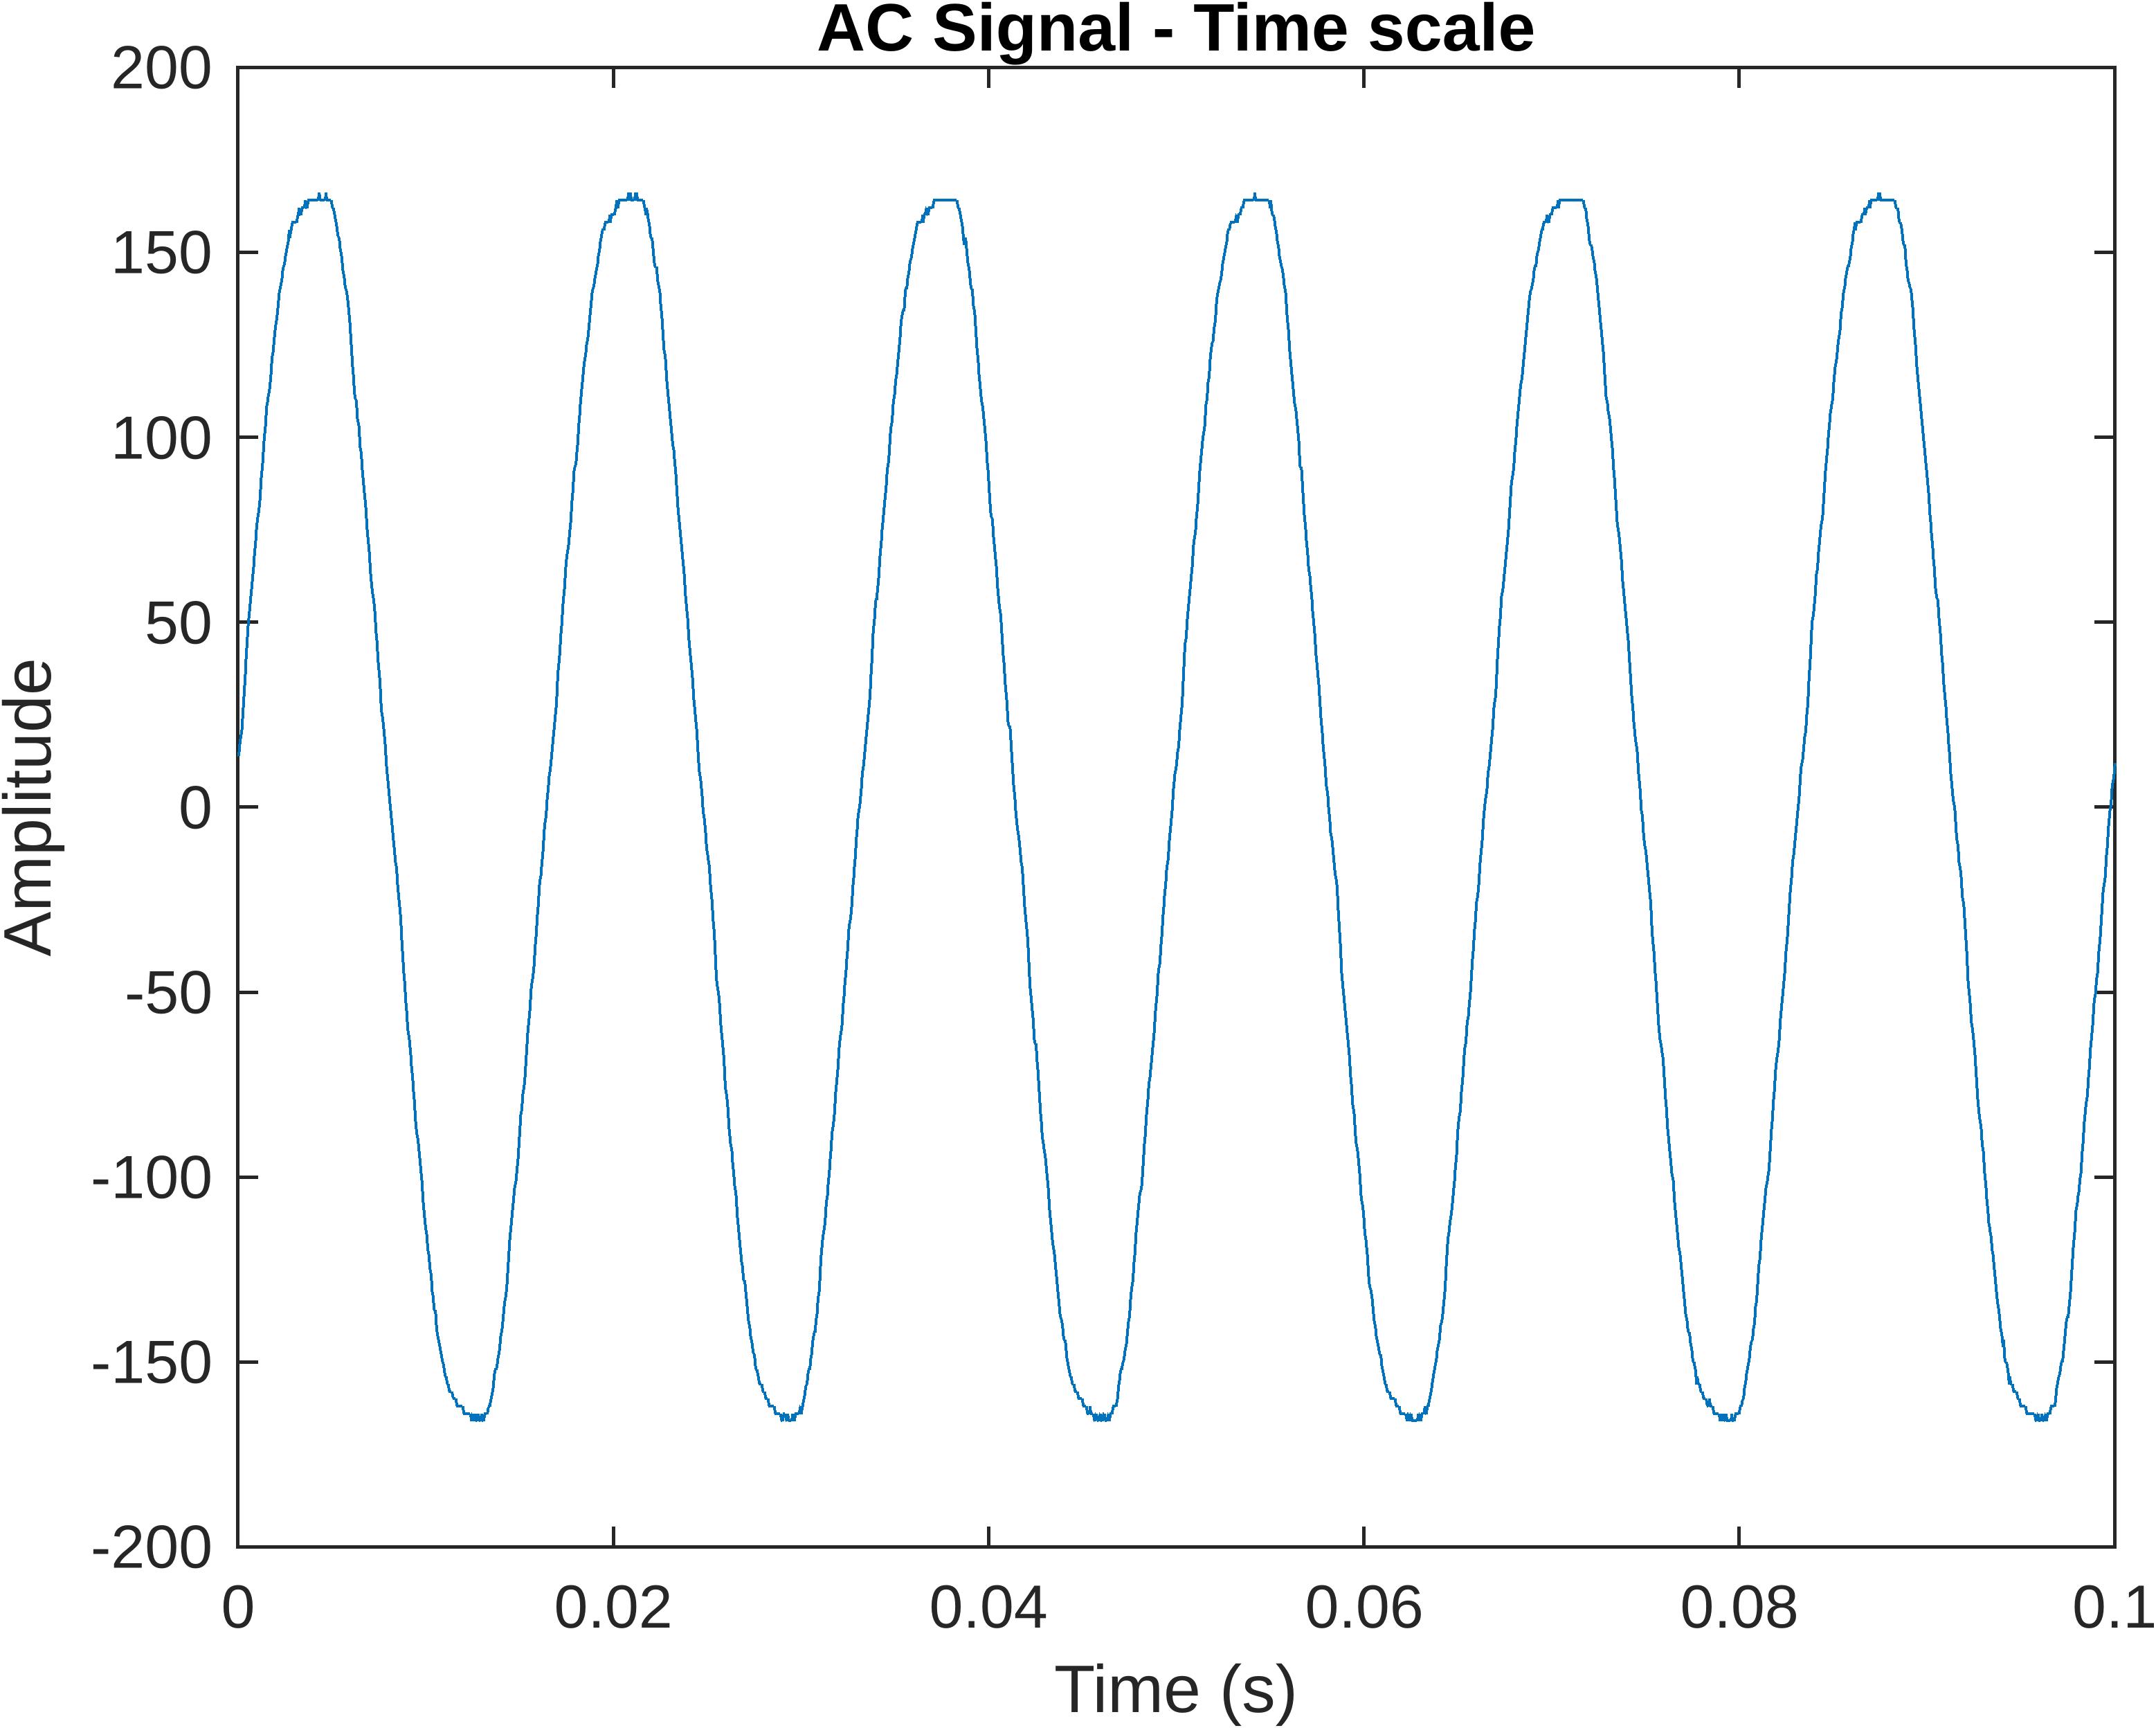
\includegraphics[width=0.5\textwidth]{signal.png}
        \caption{AC Signal with Correct Time Scale}
        \label{fig:signal}
    \end{figure}

    \item Plotting the signal in the frequency domain using \texttt{fft}, we get the result shown in \autoref{fig:fft_signal}.

    \begin{figure}[ht!]
        \centering
        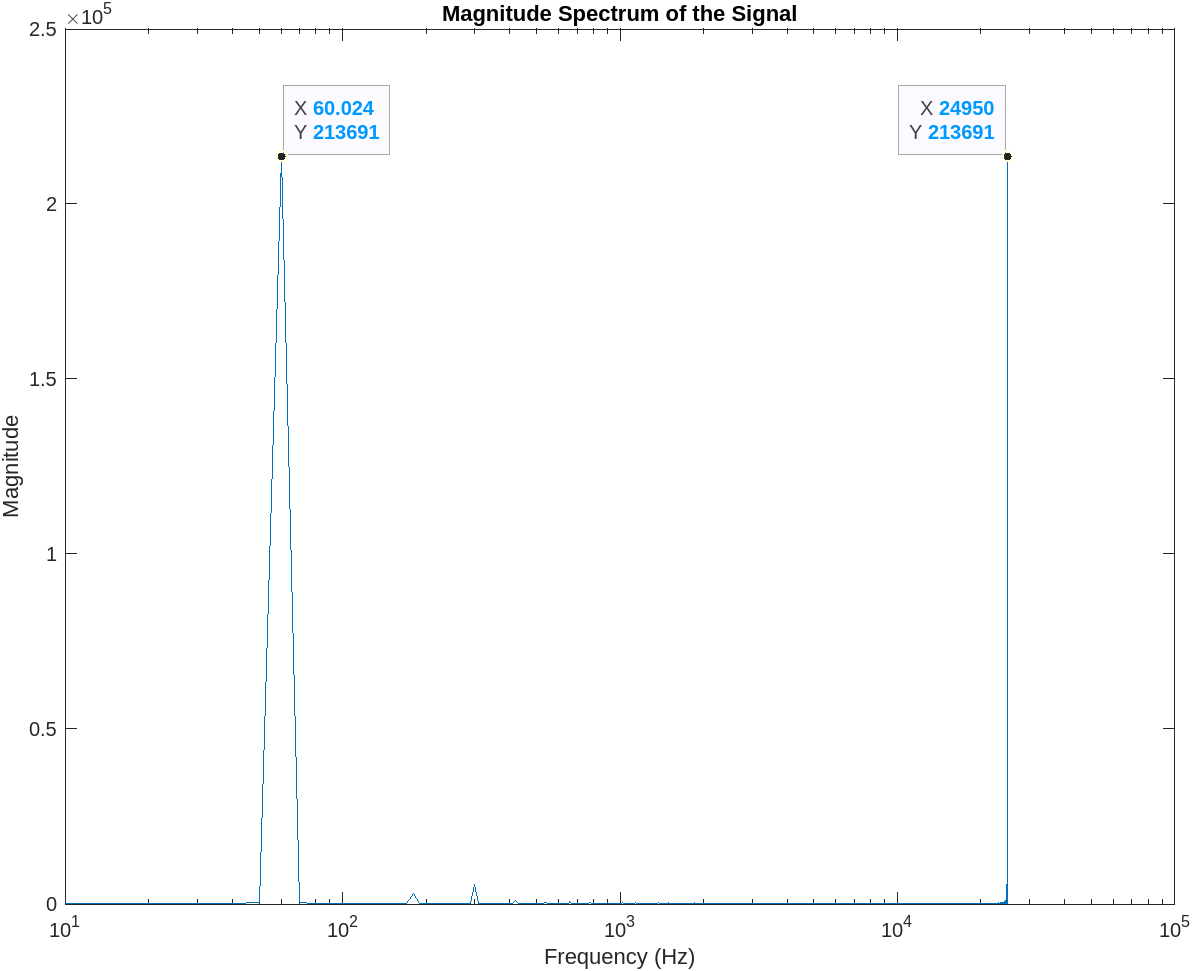
\includegraphics[width=0.5\textwidth]{fft.png}
        \caption{Frequency Domain of AC Signal}
        \label{fig:fft_signal}
    \end{figure}

    The result is as expected given that the signal is an approximate sine-wave with a frequency of 60 Hz. The frequency domain plot shows two peaks, one at 60 Hz, and the other at 24950 Hz. This is due to the symmetry of the FFT output, and if centered at 12.5 kHz, the two peaks would be shown at ~-12.5 kHz and 12.5 kHz. A log scale is used for the x-axis to better show the peaks. 

    \item To turn on a vacuum when the heavy load is on, we can detect the changes in frequencies of the signal before and after the heavy load is turned on. An RC circuit can be designed to detect the change and connect it to the relay that controls the vacuum. 

    Plotting the magnitude, in decibles, of the FFT of the two signals, we get the result shown in \autoref{fig:fft_mag}.

    \begin{figure}[ht!]
        \centering
        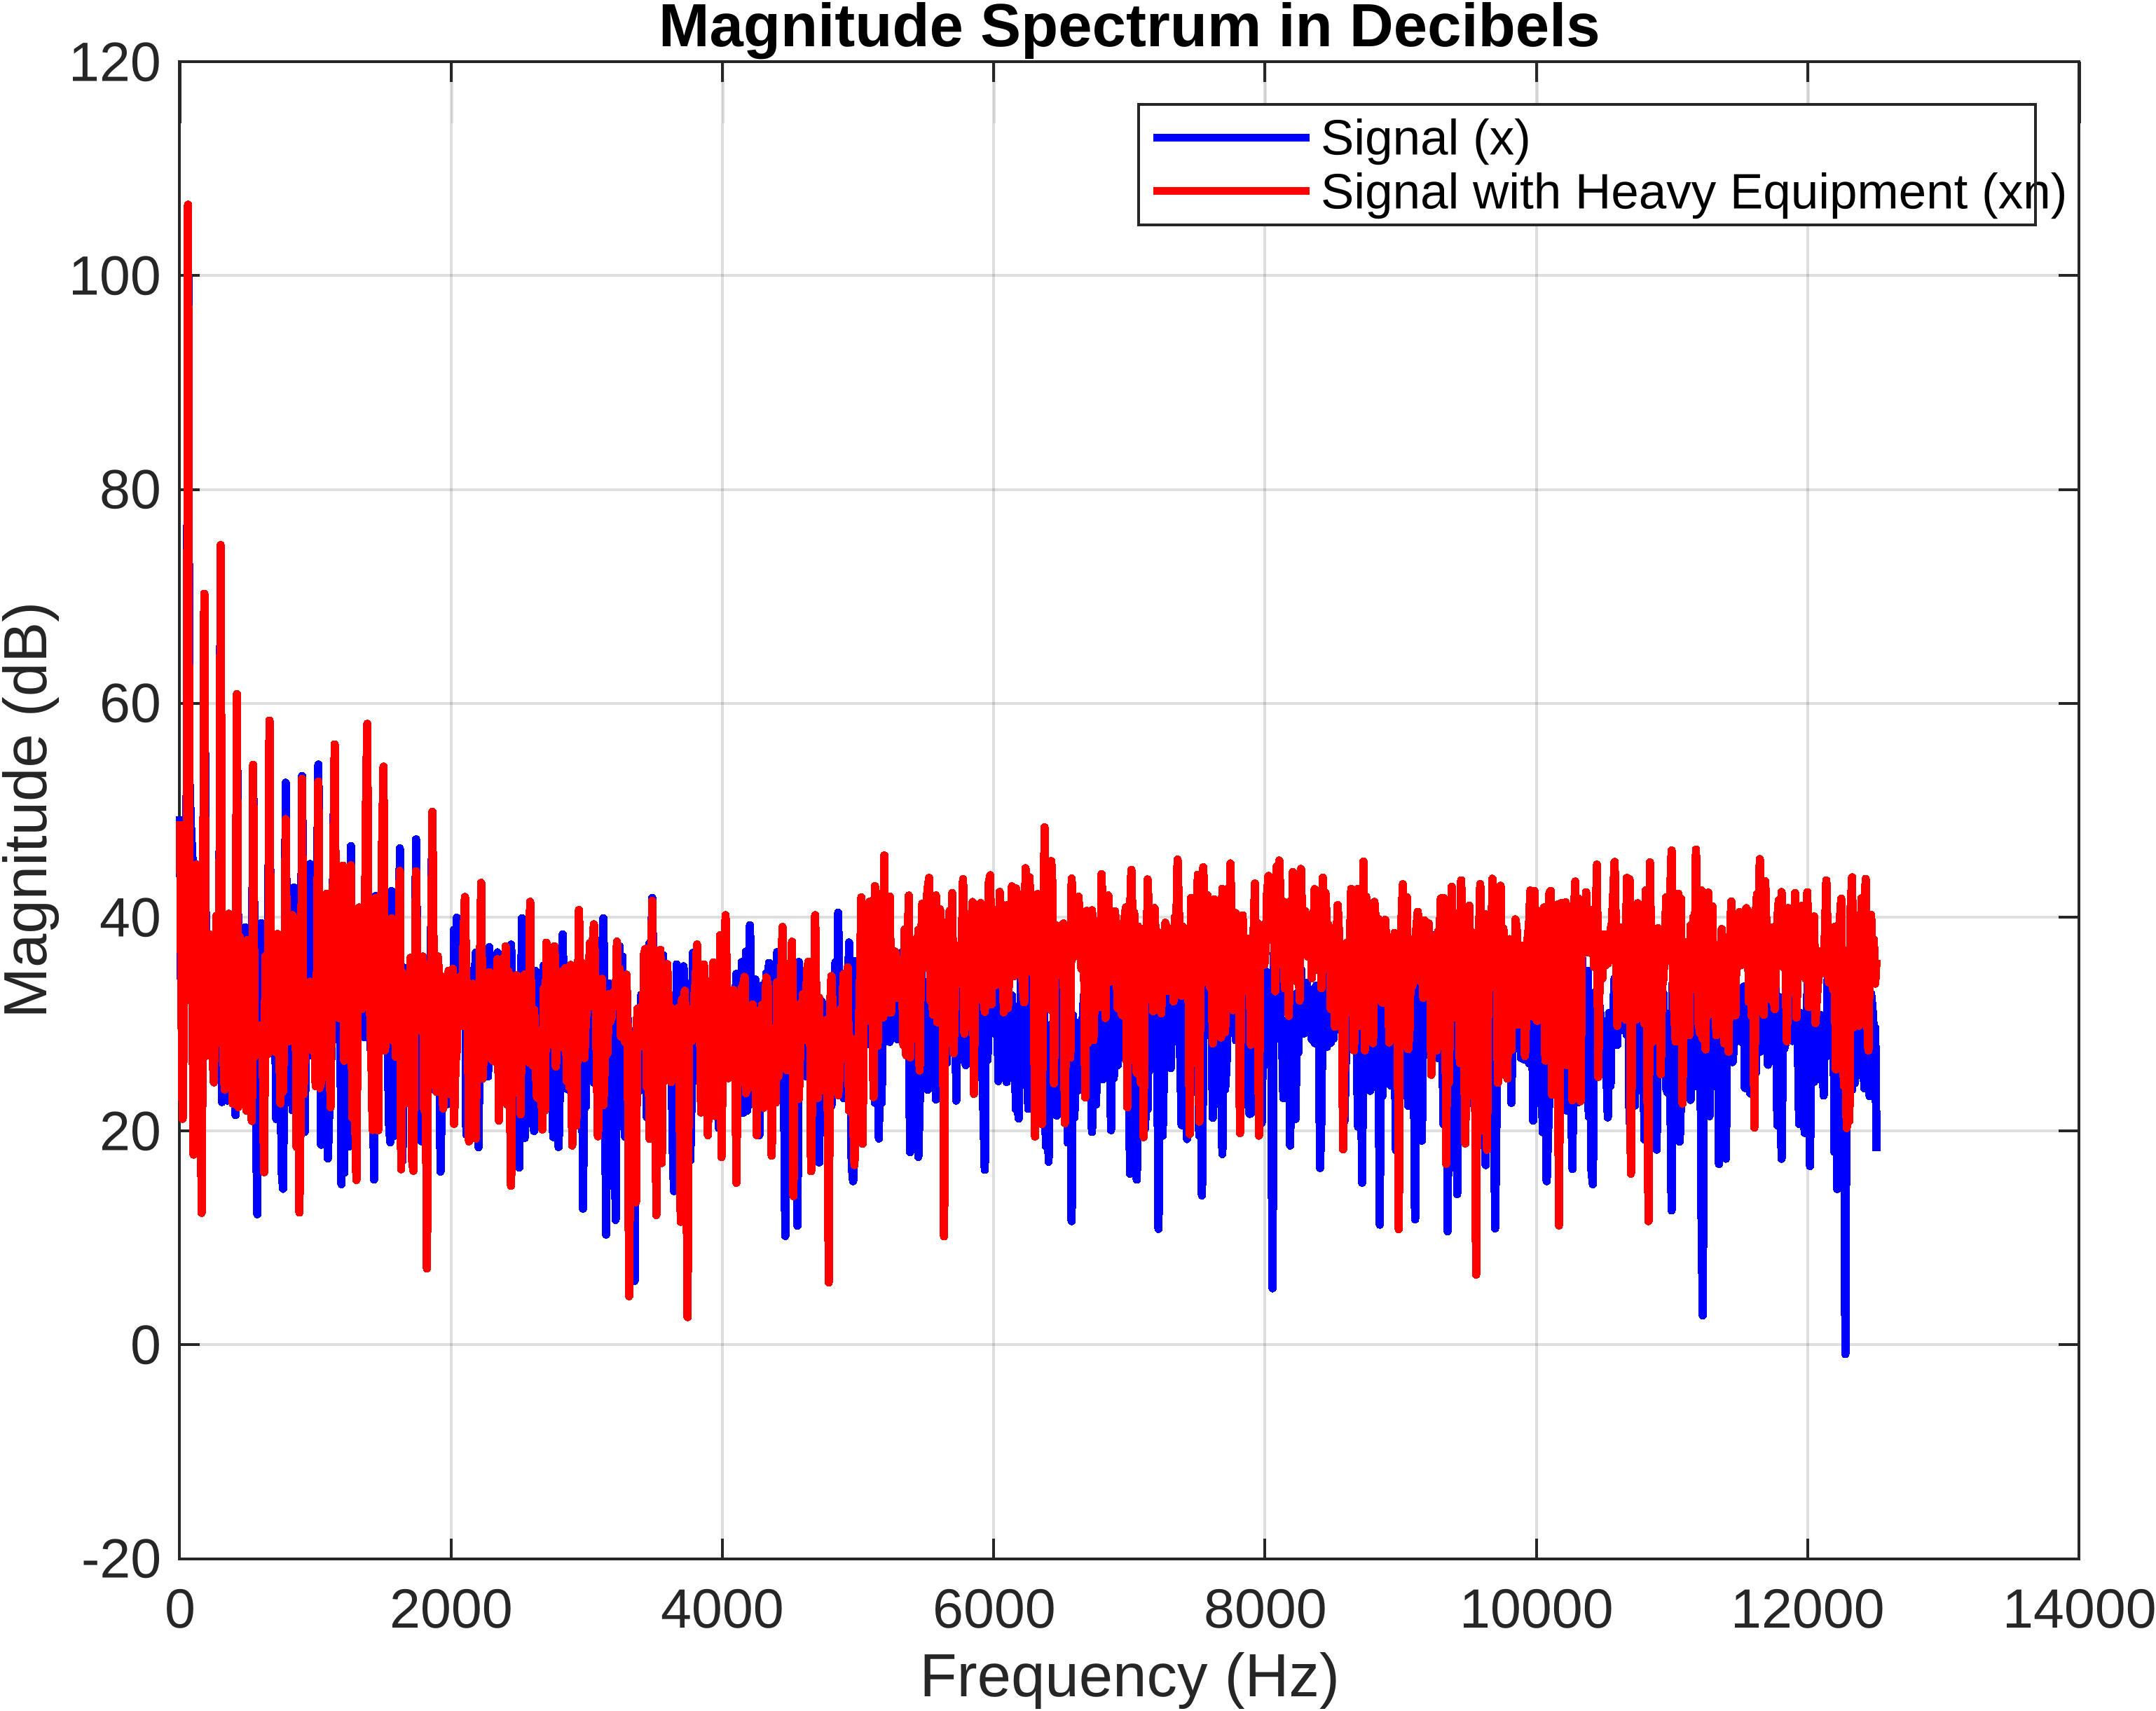
\includegraphics[width=0.5\textwidth]{fft_compare.png}
        \caption{Magnitude of FFT of AC Signal}
        \label{fig:fft_mag}
    \end{figure}

    We can see that at higher frequencies, the signal with the machine on dominates and we can design an high-pass RC filter to detect these frequencies.

    We can pick the cutoff frequency of the filter to be around 10 kHz. This will allow the signal with the machine on to pass through, while filtering out the signal with the machine off. The values of the resistor and capacitor can be calculated using the following formula:
    \begin{align*}
        f_c &= \frac{1}{2\pi RC} \\
        \text{Let } f_c &= 10 \text{ kHz} \\
        \text{Let } R &= 10 \text{ k}\Omega \\
        \text{Then } C &= \frac{1}{2\pi \times 10 \times 10^3 \times 10 \times 10^3} = 1.59 \times 10^{-6} \text{ F}\\
        \text{Choose } C &= 1.5 \mu F \\
    \end{align*}

    With these values for the resistor and capacitor, we can read the output of the resistor, and then connect it to a amplifier to drive the relay that controls the vacuum.

\end{enumerate}

\section{Problem 3}

\textbf{3.1-6}
We have:
\[
    x[n] = \begin{cases}
        \left(\frac{1}{3}\right)^n & \text{if } n \geq 0 \\
        A^n & \text{if } n < 0
    \end{cases}
\]
Too determine the power and energy, we can use the following general equations:

For energy:
\begin{align*}
    E_x &= \sum_{n=-\infty}^{\infty} |x[n]|^2 = \sum_{n=-\infty}^{-1} |A^n|^2 + \sum_{n=0}^{\infty} \left(\frac{1}{3}\right)^{2n} \\ 
    &= \sum_{m=1}^{\infty} |A|^{-2m} + \sum_{n=0}^{\infty} \left(\frac{1}{9}\right)^n = \sum_{m=1}^{N} \frac{1}{A^{2m}} + \frac{1}{1 - \frac{1}{9}} \\
    &= \left(\sum_{m=0}^{N} \frac{1}{A^{2m}}\right) - 1 + \frac{9}{8} \\
    &= \sum_{m=0}^{N} \left(\frac{1}{A^2}\right)^m + \frac{1}{8}
\end{align*}
If $|A| \leq 1$, then the sum will diverge to infinity as $1/A^2 \geq 1$. If $|A| > 1$, then the sum will converge to a finite value. Therefore:
\begin{align*}
    E_x &= \begin{cases}
        \infty & \text{if } |A| \leq 1 \\
        \frac{1}{1 - \frac{1}{A^2}} + \frac{1}{8} & \text{if } |A| > 1
    \end{cases}
\end{align*}

\begin{enumerate}[label=\alph*.]
    \item Determine the energy $E_x$ and power $P_x$ of $x[n]$ if A = 1/2.
    
    Since $|A| < 1$, and using the results from above, the energy of the signal is infinite, that is:
    \begin{align*}
        E_x &= \infty
    \end{align*}

    The power can be found as follows:
    \begin{align*}
        P_x &= \lim_{N \to \infty} \frac{1}{2N + 1} \sum_{n=-N}^{N} |x[n]|^2 \\
        &= \lim_{N \to \infty} \frac{1}{2N + 1} \left(\sum_{n=-N}^{-1} \left(\frac{1}{2}\right)^{2n} + \sum_{n=0}^{N} \left(\frac{1}{3}\right)^{2n}\right) \\
        &= \lim_{N \to \infty} \frac{1}{2N + 1} \left(\sum_{n=-N}^{-1} \left(\frac{1}{4}\right)^{n} + \sum_{n=0}^{N} \left(\frac{1}{9}\right)^{n}\right) \\   
        &= \lim_{N \to \infty} \frac{1}{2N + 1} \left(\sum_{m=1}^{N} 4^m + \sum_{n=0}^{N} \left(\frac{1}{9}\right)^{n}\right) \\
    \end{align*}
    We can use the following two formulas to find the sum of the two series:
    \begin{align*}
        \sum_{m=1}^{N} 4^m = 4 + 4^2 + 4^3 + \ldots + 4^N &= \frac{4(4^N - 1)}{4 - 1} = \frac{4^{N+1} - 4}{3} \\
        \sum_{n=0}^{N} \frac{1}{9^n} &= \frac{1 - \frac{1}{9^{N+1}}}{1 - \frac{1}{9}} = \frac{9}{8}\left(1 - \frac{1}{9^{N+1}}\right)
    \end{align*}

    We now have the following:
    \begin{align*}
        P_x &= \lim_{N \to \infty} \frac{1}{2N + 1} \left(\frac{4^{N+1} - 4}{3} + \frac{9}{8}\left(1 - \frac{1}{9^{N+1}}\right)\right) \\
    \end{align*}
    Now as $N \to \infty$, the term $\frac{1}{9^{N+1}}$ goes to 0, and the $4^{N+1}$ term grows very large. This means that the power of the signal is infinite, that is:
    \[
        P_x \rightarrow \infty
    \]
    \item Determine the energy $E_x$ and power $P_x$ of $x[n]$ if A = 1.
    
    Since $|A| = 1$, and using the results from above, the energy of the signal is infinite, that is:
    \begin{align*}
        E_x &= \infty
    \end{align*}

    The power can be found as follows:
    \begin{align*}
        P_x &= \lim_{N \to \infty} \frac{1}{2N + 1} \sum_{n=-N}^{N} |x[n]|^2 \\
        &= \lim_{N \to \infty} \frac{1}{2N + 1} \left(\sum_{n=-N}^{-1} 1 + \sum_{n=0}^{N} \left(\frac{1}{3}\right)^{2n}\right) \\
        &= \lim_{N \to \infty} \frac{1}{2N + 1} \left(\sum_{n=-N}^{-1} 1\right) + 
        \lim_{N \to \infty} \frac{1}{2N+1}\left(\sum_{n=0}^{N} \left(\frac{1}{9}\right)^{n}\right)\\
    \end{align*}
    The second term, as N grows large will approach 0, so we can disregard and focus on the first term.
    \begin{align*}
        P_x &= \lim_{N \to \infty} \frac{1}{2N + 1} \left(\sum_{n=-N}^{-1} 1\right) \\
        &= \lim_{N \to \infty} \frac{1}{2N + 1} \left(\sum_{n=1}^{N} 1\right) \\
        &= \lim_{N \to \infty} \frac{1}{2N + 1} \left(N\right) \\
        &= \lim_{N \to \infty} \frac{N}{2N + 1} \\
        &= \frac{1}{2}
    \end{align*}

    \item Determine the energy $E_x$ and power $P_x$ of $x[n]$ if A = 2.

    Since $|A| > 1$, and using the results from above, the energy of the signal is finite, that is:
    \begin{align*}
        E_x &= \frac{1}{1 - \frac{1}{A^2}} + \frac{1}{8} = \frac{1}{1 - \frac{1}{4}} - \frac{1}{8} = \frac{4}{3} + \frac{1}{8} = \frac{35}{24}
    \end{align*}

    The power can be found as follows:
    \begin{align*}
        P_x &= \lim_{N \to \infty} \frac{1}{2N + 1} \sum_{n=-N}^{N} |x[n]|^2 \\
        &= \lim_{N \to \infty} \frac{1}{2N + 1} \left(\sum_{n=-N}^{-1} 2^{2n} + \sum_{n=0}^{N} \left(\frac{1}{3}\right)^{2n}\right) \\
        &= \lim_{N \to \infty} \frac{1}{2N + 1} \left(\sum_{n=-N}^{-1} 2^{2n}\right) + 
        \lim_{N \to \infty} \frac{1}{2N+1}\left(\sum_{n=0}^{N} \left(\frac{1}{9}\right)^{n}\right)\\
    \end{align*}
    Similar to the previous part, the second term will approach 0 as N grows large, so we can disregard it.

    \begin{align*}
        P_x &= \lim_{N \to \infty} \frac{1}{2N + 1} \left(\sum_{n=-N}^{-1} 4^n\right) \\
        &= \lim_{N \to \infty} \frac{1}{2N + 1} \left(\sum_{n=1}^{N} 4^{-n}\right) \\
    \end{align*}
    We can use the following formula to find the sum of the series:
    \begin{align*}
        \sum_{n=1}^{N} 4^{-n} = \frac{1}{4} + \frac{1}{4^2} + \frac{1}{4^3} + \ldots + \frac{1}{4^N} &= \frac{1}{3}\left(1 - \frac{1}{4^N}\right)
    \end{align*}
    We can now substitute this back into the equation for $P_x$:
    \begin{align*}
        P_x &= \lim_{N \to \infty} \frac{1}{2N + 1} \left(\frac{1}{3}\left(1 - \frac{1}{4^N}\right)\right) \\
        &= \lim_{N \to \infty} \frac{1}{2N + 1} \left(\frac{1}{3} - \frac{1}{3 \cdot 4^N}\right) \\
        &= 0
    \end{align*}

\end{enumerate}

\textbf{3.3-3}
\autoref{fig:signals} shows the plots of the provided signals. The code to generate these signals is provided in the appendix at \autoref{code:plot_gen}.
\begin{figure}[ht!]
    \centering
    \begin{subfigure}[b]{0.3\textwidth}
        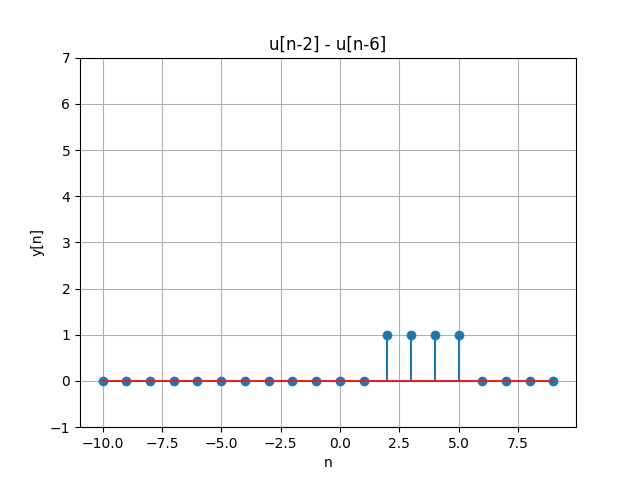
\includegraphics[width=\textwidth]{plot1.png}
        \caption{$u[n-2]-u[n-6]$}
    \end{subfigure}
    \begin{subfigure}[b]{0.3\textwidth}
        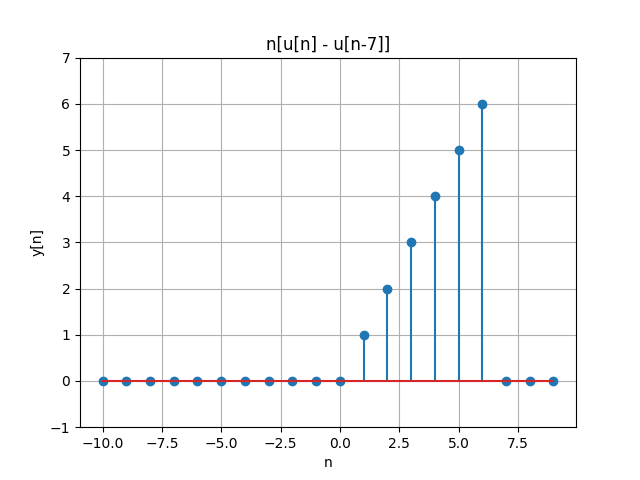
\includegraphics[width=\textwidth]{plot2.png}
        \caption{$n(u[n]-u[n-7])$}
    \end{subfigure}
    \begin{subfigure}[b]{0.3\textwidth}
        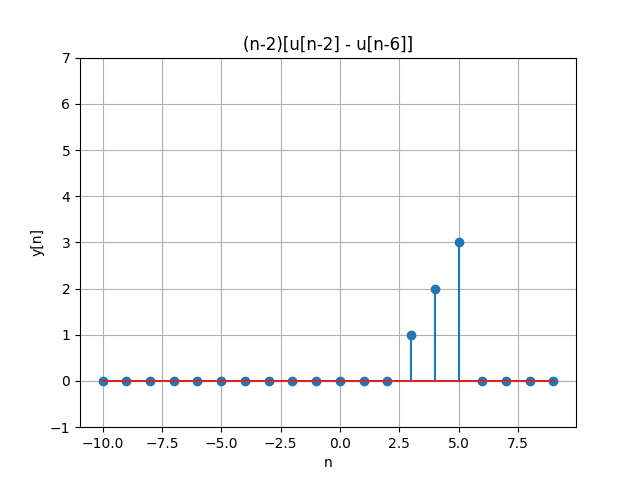
\includegraphics[width=\textwidth]{plot3.png}
        \caption{$(n-2)(u[n-2]-u[n-6])$}
    \end{subfigure}
    \begin{subfigure}[b]{0.3\textwidth}
        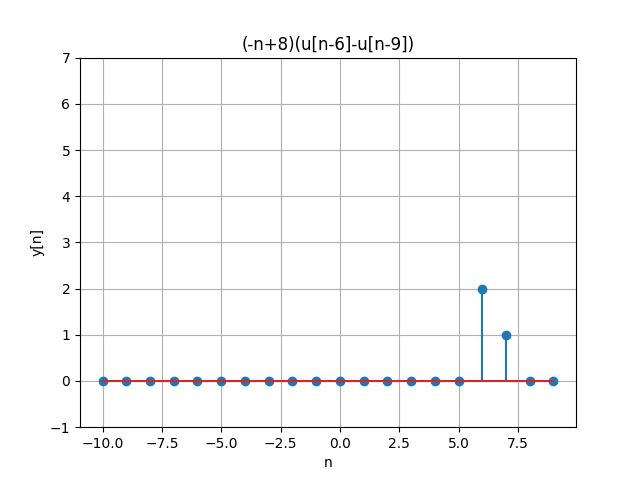
\includegraphics[width=\textwidth]{plot4.png}
        \caption{$(-n+8)(u[n-6]-u[n-9])$}
    \end{subfigure}
    \begin{subfigure}[b]{0.3\textwidth}
        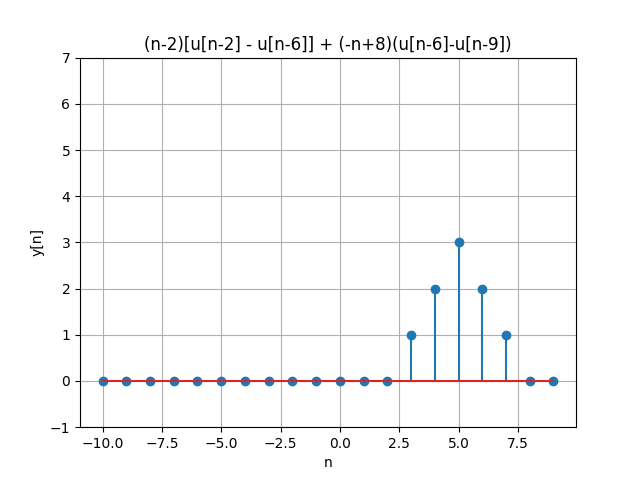
\includegraphics[width=\textwidth]{plot5.png}
        \caption{$(n-2)(u[n-2]-u[n-6])+(-n+8)(u[n-6]-u[n-9])$}
    \end{subfigure}
    \caption{Plots of various signals}
    \label{fig:signals}
\end{figure}

\textbf{3.6-1}

We have the following difference equation:
\begin{align*}
    y[n] + \frac{1}{6}y[n-1] - \frac{1}{6}y[n-2] &= \frac{1}{3}x[n] + \frac{2}{3}x[n-2]\\
    y_0[-1] = 3, &\quad y_0[-2] = -1 \\
\end{align*}

The following code can be used to output the first 10 values of $y[n]$, assuming $x[n] = u[n]$:
\newpage
\begin{lstlisting}[language=Python, label={code:p3}, caption={Python code to solve difference equation}]
def unit_step(n):
    return 1 if n >= 0 else 0

y = {}
x = {}

# Initial conditions
y[-1] = 3
y[-2] = -1

for n in range(10):
    x[n] = unit_step(n)
    x[n-2] = unit_step(n-2)
    y[n] = (-1/6) * y[n-1] + (1/6) * y[n-2] + (1/3) * x[n] + (2/3) * x[n-2]
    print(f"y[{n}] = {y[n]:.5f}")
\end{lstlisting}

Plotting the first 10 values of $y[n]$ we get the result shown in \autoref{fig:y_n}.
\begin{figure}[ht!]
    \centering
    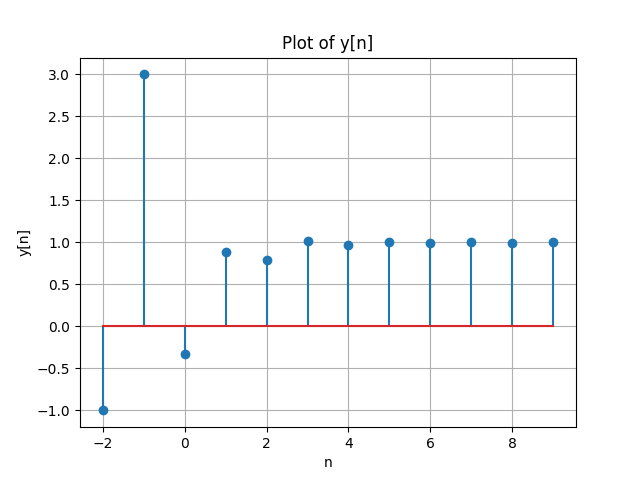
\includegraphics[width=0.5\textwidth]{p3.png}
    \caption{First 10 values of $y[n]$}
    \label{fig:y_n}
\end{figure}

\newpage
\appendix
\section{Code}
\begin{lstlisting}[language=Python, label={code:plot_gen}, caption={Python code to generate plots}]
import matplotlib.pyplot as plt
import numpy as np

def unit_step(n):
    return 1 if n >= 0 else 0

# plot 1
# u[n-2] - u[n-6]

n = np.arange(-10, 10)
y1 = np.zeros(20)
for i in range(20):
    y1[i] = unit_step(n[i] - 2) - unit_step(n[i] - 6)

plt.figure(1)
plt.stem(n, y1)
plt.title('u[n-2] - u[n-6]')
plt.xlabel('n')
plt.ylabel('y[n]')
plt.ylim(-1, 7)
plt.grid(True)
plt.savefig('/plot1.png')

# plot 2
# n[u[n] - u[n-7]]
y2 = np.zeros(20)
for i in range(20):
    y2[i] = n[i] * (unit_step(n[i]) - unit_step(n[i] - 7))

plt.figure(2)
plt.stem(n, y2)
plt.title('n[u[n] - u[n-7]]')
plt.xlabel('n')
plt.ylabel('y[n]')
plt.ylim(-1, 7)

plt.grid(True)
plt.savefig('/plot2.png')

# plot 3
# (n-2)[u[n-2] - u[n-6]]
y3 = np.zeros(20)
for i in range(20):
    y3[i] = (n[i] - 2) * (unit_step(n[i]-2) - unit_step(n[i] - 6))

plt.figure(3)
plt.stem(n, y3)
plt.title('(n-2)[u[n-2] - u[n-6]]')
plt.xlabel('n')
plt.ylabel('y[n]')
plt.ylim(-1, 7)

plt.grid(True)
plt.savefig('/plot3.png')

# plot 4
# (-n+8)(u[n-6]-u[n-9])
y4 = np.zeros(20)
for i in range(20):
    y4[i] = (-n[i] + 8) * (unit_step(n[i] - 6) - unit_step(n[i] - 9))
    
plt.figure(4)
plt.stem(n, y4)
plt.title('(-n+8)(u[n-6]-u[n-9])')
plt.xlabel('n')
plt.ylabel('y[n]')
plt.ylim(-1, 7)
plt.grid(True)
plt.savefig('/plot4.png')

# plot 5
# (n-2)[u[n-2] - u[n-6]] + (-n+8)(u[n-6]-u[n-9])
y5 = y3 + y4

plt.figure(5)
plt.stem(n, y5)
plt.title('(n-2)[u[n-2] - u[n-6]] + (-n+8)(u[n-6]-u[n-9])')
plt.xlabel('n')
plt.ylabel('y[n]')
plt.ylim(-1, 7)

plt.grid(True)
plt.savefig('/plot5.png')
\end{lstlisting}

% --------------------------------------------------------------------------------
% END BODY
% --------------------------------------------------------------------------------

\end{document}
